\chapter{Ferramenta Crickets' little leg}\label{2_ferramenta_cll}

Foi necessária a realização de um levantamento de algumas das tecnologias atuais, no contexto de aplicações \textit{Web}, de modo que fora realizado um processo de conhecimento e experimentação das mesmas, para que as atividades relacionadas ao desenvolvimento pudessem ser realizadas.

Como o público alvo que se deseja atingir são administradores que possuem sistemas baseados em famílias \textit{Unix}, pode-se levantar características em comum, encontradas em seus sistemas. Dessa maneira, se obtém o perfil das tecnologias que trabalham em conjunto na maioria dos ambientes, o que porporciona maiores chances de adesão da ferramenta. A tabela \ref{tabela:tecnologiasWeb} mostra quais são as tecnologias mais aderidas perante à comunidade, quando implantadas ferramentas em ambientes \textit{Web}:

\begin{table}[ht]
    \centering
    \caption{\label{tabela:tecnologiasWeb}Tecnologias mais empregadas em aplicações Web}

    \begin{tabular}{c c}
        \hline
        \hline

        Propósito & Tecnologia\\ [0.5ex]
        \hline

        Sistema Operacional & Família \textit{Unix}\\

        Servidor \textit{Web} & \textit{Apache}\\

        Servidor de Banco de dados & \textit{MySQL}\\

        Linguagem de \textit{Scripting} & \textit{PHP}\\ [0.1ex]
        \hline
    \end{tabular}
    \label{webapptech}
\end{table}

É importante, também, que a ferramenta seja portável, de modo que sua implantação seja facilmente realizada em ambientes que atendam aos requisitos tecnológicos básicos levantados até então. Por isso, foi constatada a necessidade de se encontrar um bom \textit{framework} de desenvolvimento \textit{Web}, que atendesse a este anseio. Para a linguagem de \textit{scripting PHP} \cite{PHP}, o \textit{framework CakePHP} \cite{CakePHP} foi escolhido, pois tem como uma das características mais marcantes, a facilidade com que as aplicações são implantadas, não tendo exigência alguma quanto à modificações na estrutura padrão do Sistema Operacional, desta forma os administradores não precisam realizar operações custosas em seus sistemas para que a ferramenta seja suportada.


\section{Tecnologias envolvidas}

Foi realizado um levantamento inicial sobre as tecnologias envolvidas no processo de desenvolvimento da ferramenta, onde serão abordadas suas principais características. Alguns contrapontos foram encontrados em sua definição, principalmente com relação à linguagem de \textit{scripting} empregada e seu \textit{framework} escolhido, discutidos adiante.

Na busca por uma combinação ideal, foi necessário o entendimento sobre o ambiente escolhido para implantação e as implicações de se ter tal ferramenta disponibilizada em meio ao sistema.

\subsection{Servidor Web}

Como servidor \textit{Web}, foi escolhido o \textit{Apache} \cite{ApacheHttpd}, devido sua popularidade e uso amplamente difundido entre a comunidade de desenvolvedores e administradores de sistemas. É um dos maiores projetos em Software Livre do mundo, sendo percursor na criação da incubadora de projetos da \textit{Apache Software Foundation} \cite{ApacheSWFoundation}. Tem sido desenvolvido desde o ano de 1995 e conta com uma comunidade extremamente ativa de colaboradores, provenientes de diferentes partes de todo o mundo.

Perante o mercado e às outras soluções de servidores \textit{Web}, o \textit{Apache} ocupa uma porção de uso correspondente a aproximadamente 47\%, segundo revelam as pesquisas \cite{Netcraft} disponibilizadas periodicamente pela companhia de serviços relacionados à \textit{Internet}, \textit{Netcraft}. A figura \ref{figura:utilizacao_webservers} mostra um gráfico percentual de utilização global das tecnologias em Webservers, confirmando o servidor \textit{Web Apache}, como sendo o mais amplamente adotado em sua categoria:

\begin{figure}[H]
    \begin{center}
        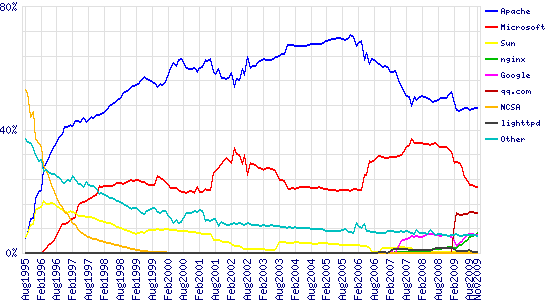
\includegraphics[scale=0.8]{./figuras/overallc.png}

        \caption{\label{figura:utilizacao_webservers}Utilização global de \textit{Webservers} \cite{Netcraft}.}
    \end{center}
\end{figure}

Sua integração com os Sistemas Operacionais baseados em famílias \textit{Unix} é suave, pois foi projetado para que se integre perfeitamente sob sua arquitetura. No momento de sua instalação, muitos sabores de distribuições baseadas no \textit{Kernel} do \textit{GNU/Linux} \cite{LinuxKernel}, por exemplo, incluem o \textit{Apache} como pacote opcional junto aos demais serviços de rede, sendo assim, uma alternativa bastante plausível de utilização, devido seu suporte praticamente nativo, além de não exigir grandes esforços em sua configuração, para que entre em ambiente de produção.

\subsection{Linguagem de Scripting}

Para que a ferramenta pudesse ser desenvolvida em ambiente \textit{Web}, foi definido que se utilizaria uma linguagem de \textit{scripting}, devido a agilidade e quantidade de recursos que simplificam muitos processos de desenvolvimento, comuns a este gênero de linguagens de programação.

Sua concepção, assume que as linguagens de \textit{scripting}, não sejam utilizadas na construção de aplicações desde toda sua base, mas que reutilizem uma série de componentes e bibliotecas previamente implementadas, possivelmente em diferentes linguagens de programação, ou ainda que controlem outros \textit{softwares} através de chamadas específicas \cite{Scripting}. Por este motivo, são amplamente empregadas nos servidores \textit{Web}, que implementam todo o processo de receber requisições \textit{HTTP} de seus clientes e repassá-las para filtros especiais, podendo estes ser interpretadores de código, e que ainda no lado do servidor, possam responder aos clientes com conteúdo estatico ou dinâmico à tais requisições, de acordo com sua entrada aliada ao conjunto de estados mapeados pela aplicação requisitada.

O servidor \textit{Web} \textit{Apache}, utiliza-se de módulos para suportar a integração com outras tecnologias, sendo que existem muitos que são implementados para suportar diversas linguagens de \textit{scripting}. O módulo mais difundido e bem suportado pelo \textit{Apache}, para este tipo de operação, é o \textit{mod\_php}, que provê acesso às funcionalidades que a linguagem de programação \textit{PHP} oferece. É distribuido juntamente aos pacotes binários e fontes do \textit{Apache}, sua configuração é praticamente nativa, não necessitando mais que pouquíssimas alterações no arquivo de configuração principal (\textit{/etc/httpd/httpd.conf}) do Apache, para que tal suporte esteja ativo.

A figura \ref{figura:linguagens_programacao}, mostra um gráfico comparativo entre o uso das linguagens de programação, sendo que é notória a importância da linguagem de scripting \textit{PHP}, já que em sua categoria lidera em primeiro lugar no uso, frente aos seus maiores concorrentes: \textit{Ruby} \cite{Ruby}, \textit{Pearl} \cite{Pearl} e \textit{Python} \cite{Python}.

\clearpage
\begin{figure}[h!tp]
    \begin{center}
        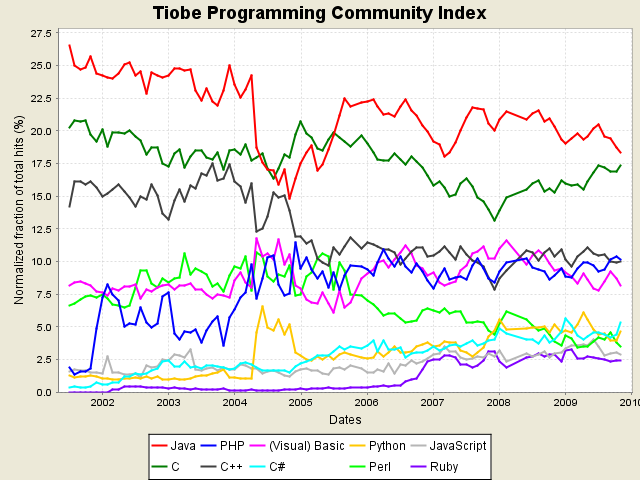
\includegraphics[scale=0.7]{./figuras/tpci_trends.png}

        \caption{\label{figura:linguagens_programacao}Utilização das linguagens de programação. \cite{Languages}}
    \end{center}
\end{figure}

\subsection{Banco de dados}

Em aplicações \textit{Web}, utilizando-se o servidor \textit{Web Apache} em conjunto com a linguagem de \textit{scripting PHP}, existe um ótimo suporte ao \textit{SGBD MySQL} \cite{php5PowerProgramming}. Trata-se de um banco de dados relacional e que oferece suporte à multiplas conexões simultâneas. \cite{MySQLreference}

Assim como as tecnologias \textit{Apache} e \textit{PHP}, também encontra-se como pacote de instalação opcional ao conjunto de serviços de rede, nas distribuições baseadas no \textit{Kernel} do \textit{GNU/Linux}. Sua aceitação é grande, em meio aos desenvolvedores \textit{Web}. De maneira similar, suporte dado tanto pela sua comunidade de desenvedores e pela sua base de usuários é extremamente vasto, o que implica em uma adesão maior pela maioria das organizações que oferecem aplicações \textit{Web}.

\subsection{Framework de desenvolvimento Web}

Para o desenvolvimento de aplicações \textit{Web}, é amplamente utilizado o auxílio que os \textit{frameworks} oferecem, pois muitos processos repetitivos são automatizados, fazendo com que o desenvolvimento se dê de maneira mais rápida e esteja menos suscetível a erros de implementação, oferecendo aos desenvolvedors níveis consideráveis de abstração de seus problemas, permitindo que se concentrem integralmente na lógica de negócios envolvida em seus projetos.

Levando-se em considerações o conjunto de tecnologias envolvidas, optou-se pela utilização do \textit{framework CakePHP}. Essa decisão foi guiada após o estudo de outra tecnologia, proposta anteriormente ao início de seu desenvolvimento.

Fora proposto no plano de estágio, a utilização da linguagem de programação \textit{Python}, em conjunto ao \textit{framework} de desenvolvimento \textit{Web Django} \cite{Django}, que basicamente, proporciona o desenvolvimento rápido de aplicações \textit{Web} seguindo o \textit{design pattern MVC} na organização dos sistemas desenvolvidos. No entanto, como requisito principal de funcionamento, tal framework necessita obrigatoriamente que seja instituído um processo que envolve modificações na hierarquia do Sistema Operacional, através de sua instalação. Isso nos remete à uma das características desejadas para a ferramenta \textit{Cricket's little leg}: que a portabilidade seja facilitada ao máximo, de acordo com o perfil mais comum entre ambientes de produção e desenvolvimento \textit{Web}. Como nem todos os sistemas administrados requerem que a linguagem de \textit{scripting Python} seja utilizada em conjunto ao ambiente \textit{Web} e, ainda sim, é incomum que nestes ambientes sejam empregadas tecnologias como \textit{Django}, optou-se pela substituição deste \textit{framework} por algum que seja tecnologicamente equivalente e que atenda ao requisito de portabilidade, desejado desde o início da concepção da ferramenta.

O \textit{CakePHP} é um \textit{framework} que atende perfeitamente esta necessidade específica, sendo equivalente até mesmo em termos de arquitetura empregada na base do \textit{framework}. Tem como vantagem principal, relativa à portabilidade, de poder ser empacotado junto à aplicação desenvolvida, e desempacotado dentro do diretório que o \textit{Apache} utiliza para servir às requisições realizadas por seus clientes, sem que seja necessária a instalação de softwares adicionais para o seu pleno funcionamento em ambiente de produção.

Pelas circunstâncias e motivos apresentados, justifica-se a troca de \textit{frameworks}, pois esta foi realizada em prol da satisfação do requisito de portabilidade, o que visa estimular ainda mais a adesão da ferramenta por parte dos administradores de sistemas que possuem, de maneira praticamente nativa, um ambiente propício e compatível ao apresentado até aqui.

\section{Estrutura}

O \textit{Crickets' little leg} foi projetado para se comportar de acordo com os padrões estabelecidos pelo \textit{Design Pattern MVC} \cite{MVC}, em conjunção às convenções empregadas no \textit{framework} de desenvolvimento \textit{Web CakePHP}.

O \textit{Design Pattern MVC} consiste de três camadas principais:
\begin{itemize}
    \item \textbf{M}odel: responsável pelos dados da aplicação, são compreendidos pelo modelo, bancos de dados, arquivos em disco, dados em memória, enfim, toda e qualquer forma de fonte que contenha os dados consultados e gravados pela aplicação.

    \item \textbf{V}iew: a camada de apresentação, trata-se de como os dados serão dispostos. Em uma aplicação \textit{Web}, consiste de uma página contento elementos \textit{HTML}, \textit{CSS}, possivelmente \textit{Javascript} e \textit{XML}, em conjunto aos dados processados no lado do servidor por uma linguagem de scripting, que no caso é a \textit{PHP}.

    \item \textbf{C}ontroller: resposável pelo fluxo de execução da aplicação, desde as requisições realizadas pelos navegadores dos clientes, até o processamento interno das mesmas, passando pela camada de modelo e pela disposição final dos dados possivelmente processados, na camada de visão.
\end{itemize}

A figura \ref{figura:MVC}, apresenta de maneira esquemática, como se dá a ligação entre as camadas \textit{MVC}:

\clearpage
\begin{figure}[h!tp]
    \begin{center}
        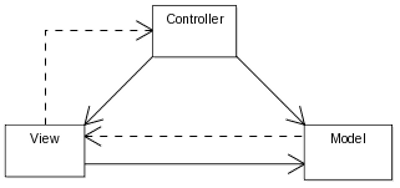
\includegraphics[scale=1]{./figuras/ModelViewControllerDiagram.png}

        \caption{\label{figura:MVC}Diagrama representativo do \textit{Design Pattern MVC}.}
    \end{center}
\end{figure}

Com esta abordagem, a construção de aplicações \textit{Web} torna-se extremamente simplificada, fornecendo diretivas suficientes para que sua construção seja rápida e que tragam ao desenvolvedor um processo bem definido em sua codificação, possibilitando uma concentração mais aplicada à resolução da lógica proposta pelo problema que se deseja resolver.

O fluxo de utilização do \textit{Design Pattern MVC}, pelo framework de desenvolvimento \nohyphens{\textit{CakePHP}} é exemplificado pela figura \ref{figura:MVC_CakePHP}

\begin{figure}[h!tp]
    \begin{center}
        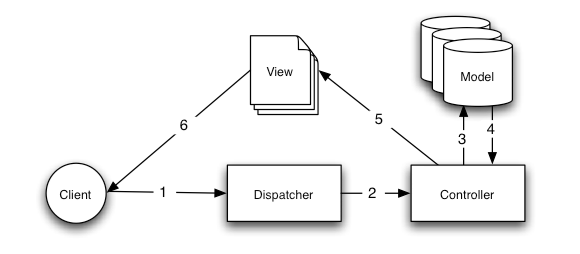
\includegraphics[scale=0.8]{./figuras/basic_mvc_cake.png}

        \caption{\label{figura:MVC_CakePHP}\textit{CakePHP} e o \textit{Design Pattern MVC}.}
    \end{center}
\end{figure}

Através dos ítens numerados, pode-se traçar um perfil padrão para todas as requisições realizadas para as aplicações que fazem uso do \textit{CakePHP}:
\begin{enumerate}
    \item O cliente realiza a requisição.

    \item O mecanismo chamado \textit{dispatcher}, permite que o processo de passagem de uma mensagem para uma sequência específica de código, ou método, seja realizado em tempo de execução. Verifica a \textit{URL} e seus dados, acionando uma chamada em um método de um objeto específico, instanciado como controlador.

    \item O controlador escolhido pelo \textit{dispatcher}, passa o fluxo de execução, para o modelo designado pela chamada recebida, com os dados necessários para sua execução, caso sejam necessários.

    \item O modelo responde ao controlador com os dados requisitados, processados após serem extraídos da fonte de dados padrão da aplicação.

    \item O controlador encaminha os dados recebidos à visão, aplicando filtros para ajustes finais, caso sejam necessários.

    \item A visão renderiza os dados, junto aos elementos comuns, encontrados em páginas \textit{Web}, como tabelas e campos de formulários, sendo assim visualizados no navegador do cliente, que antes fizera a requisição inicial.
\end{enumerate}

\clearpage
\section{Características}

As características principais da ferramenta são compreendidas pelos ítens denominados a seguir:

\begin{itemize}
    \item Utilização do mecanismo básico de autenticação \cite{BasicAuth}, implementado nativamente pelo \textit{Apache} e suportado pela grande maioria dos navegadores \textit{Web} existentes no mercado, no intuito de facilitar a implementação da parte de \textit{logon} no sistema, visando acima de tudo, a simplicidade por meio da reutilização de componentes.

    \begin{figure}[h!tp]
        \centering
        \fbox{
            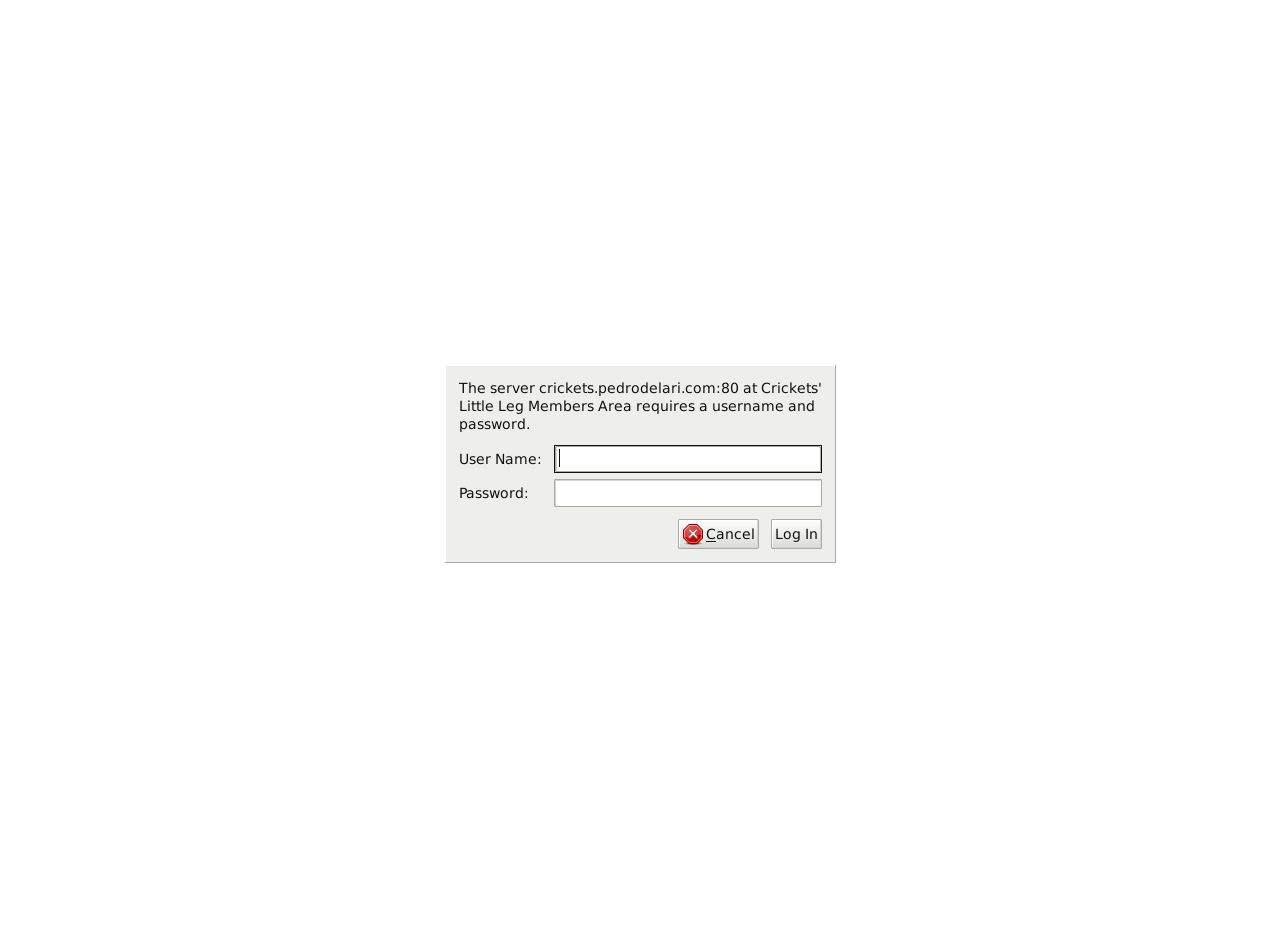
\includegraphics[scale=0.5]{./figuras/crickets_http_auth.png}
        }
        \caption{\label{figura:crickets_http_auth} Autenticação básica \textit{HTTP}.}
    \end{figure}

    \clearpage
    \item Visualização dos ataques de dicionário ao serviço \textit{SSH} sofridos no servidor local, a partir da interpretação dos dados gravados em \textit{log}, bastando informar o path onde estão localizados.

    \item Visualização dos ataques de dicionário ao serviço \textit{SSH} sofridos em qualquer outro servidor, a partir do upload de seus arquivos de \textit{log}.

    \begin{figure}[h!tp]
        \centering
        \fbox{
            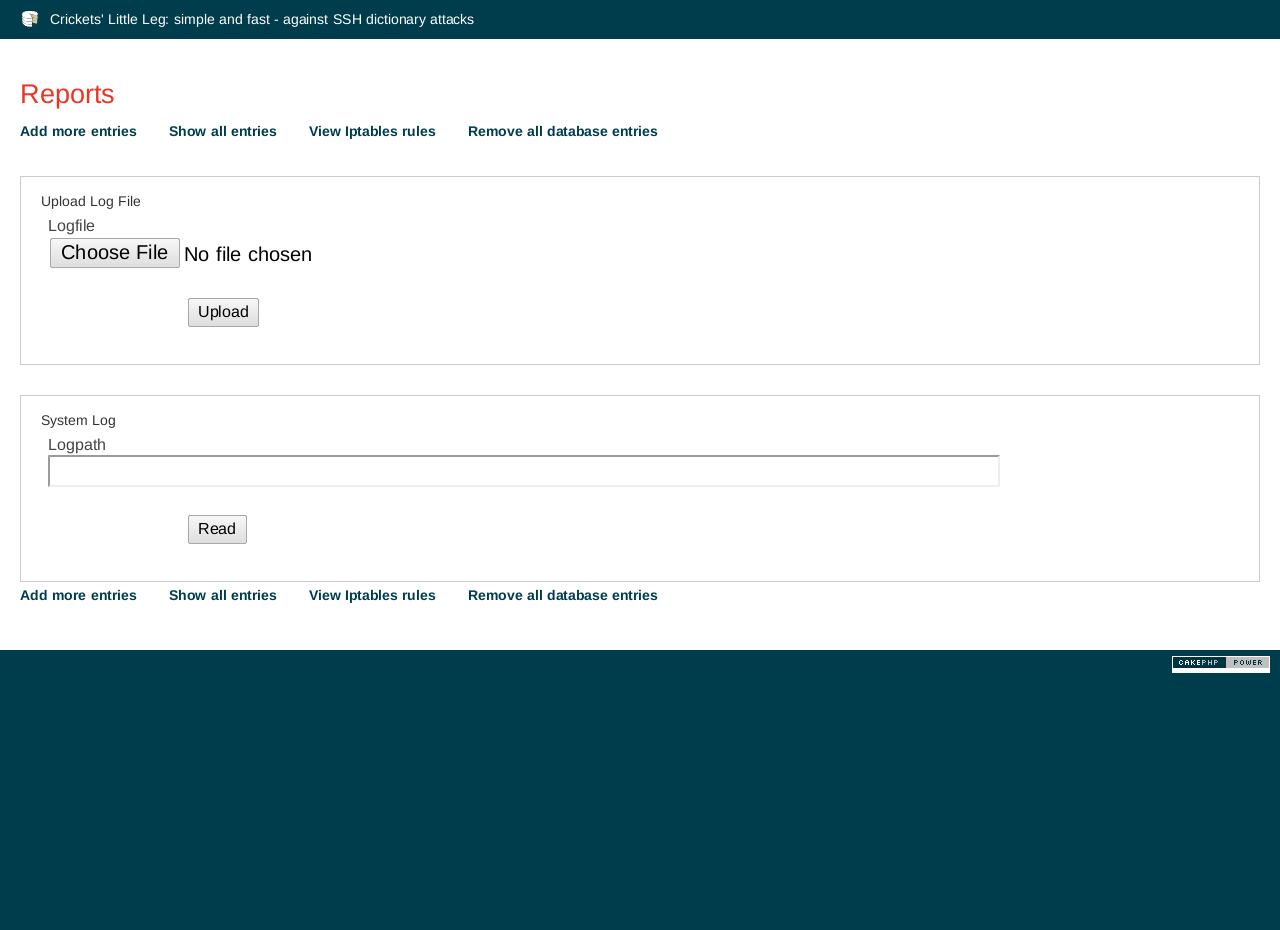
\includegraphics[scale=0.5]{./figuras/crickets_logs.png}
        }
        \caption{\label{figura:crickets_logs} Seleção da fonte de dados.}
    \end{figure}

    \clearpage
    \item Tela provida com paginação básica, contendo os dados relativos aos ataques sofridos, após o processamento dos arquivos de \textit{log}.

    \begin{figure}[h!tp]
        \centering
        \fbox{
            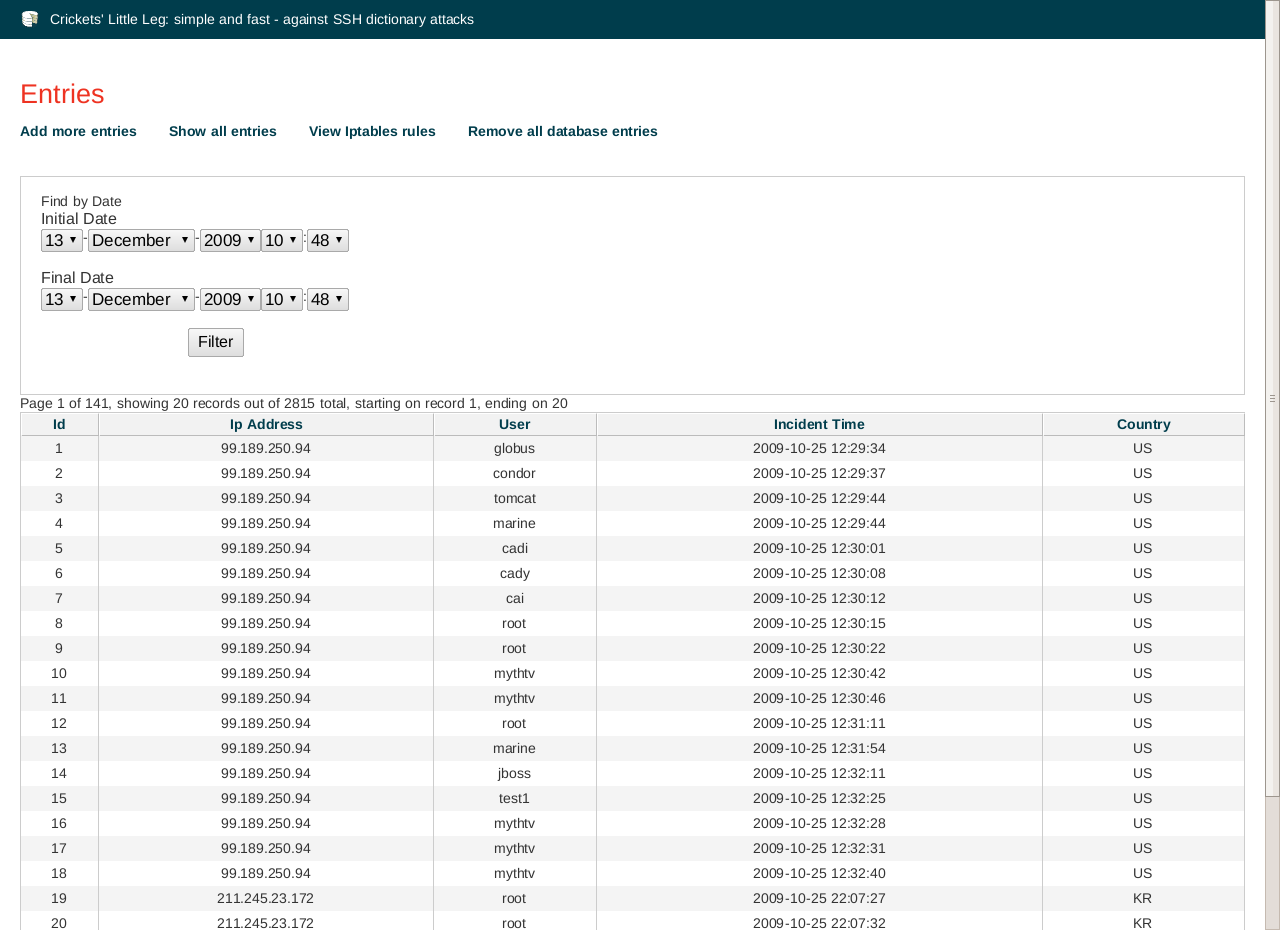
\includegraphics[scale=0.5]{./figuras/crickets_entries.png}
        }
        \caption{\label{figura:crickets_entries} Dados extraídos dos logs.}
    \end{figure}

    \clearpage
    \item Possibilidade de geração de regras de \textit{Iptables}, capazes de barrar ataques deste gênero, com base nos endereços de \textit{IP} pertencentes aos atacantes identificados pela interpretação dos registros contidos no arquivo de \textit{log}.

    \begin{figure}[h!tp]
        \centering
        \fbox{
            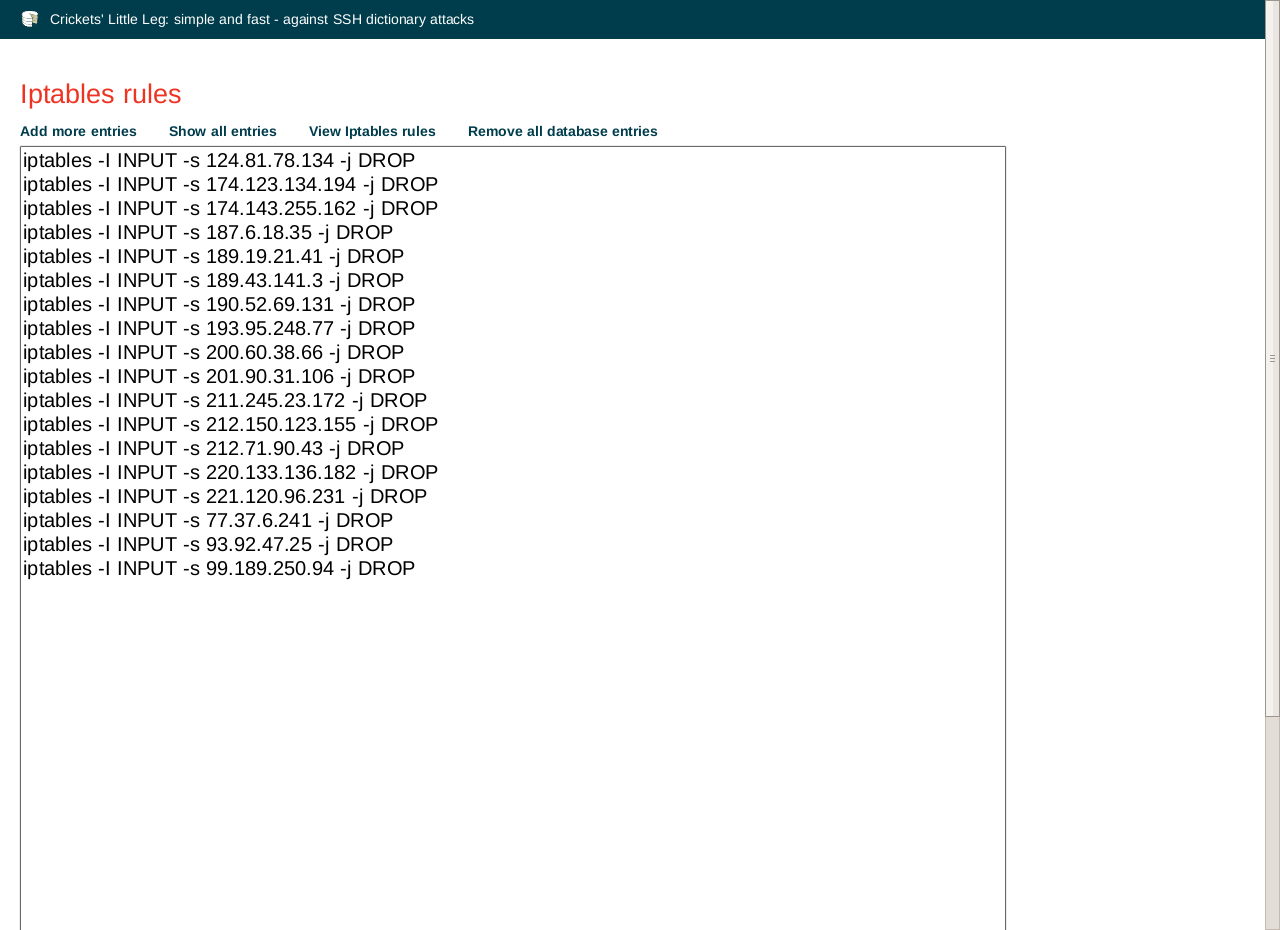
\includegraphics[scale=0.5]{./figuras/crickets_iptables.png}
        }
        \caption{\label{figura:crickets_iptables} Regras de Iptables geradas a partir dos dados extraídos pela ferramenta.}
    \end{figure}

\end{itemize}

Um exemplo reduzido do log extraído de um caso real de ataques por dicionário, realizado para a elaboração da ferramenta, é mostrado no anexo \ref{anexo:log_filtrado}

Para a elaboração da ferramenta, utilizou-se um computador que fora exposto a ataques de dicionário ao serviço \textit{SSH}. Os dados coletados a partir dos ataques foram armazenados em logs, tendo sido utilizados como base para a identificação de padrões nos arquivos. A identificação dos dados foi realizada por meio de expressões regulares \textit{taggeadas}. Cada campo relevante nas linhas escolhidas do arquivo de logs, recebeu uma marca correspondente, sendo extraído e armazenado posteriormente, no banco de dados.

Uma questão abordada durante a fase de idealização do projeto, era a capacidade de gerar alertas aos administradores do sistema. Como a ferramenta teve seu desenvolvimento voltado exclusivamente para a visualização das informações em forma de relatório, essa característica foi eliminada, por fugir ao escopo de sua atuação. Tal tarefa seria exclusiva à Sistemas de Detecção de Intrusão e por este motivo, foi considerada semanticamente incompatível com o propósito do projeto, justificando assim, o motivo pelo qual tal característica fora eliminada do processo de desenvolvimento.

\section{Localização do atacante}

A ferramenta é capaz de localizar os países de onde partiram os ataques ao servidor analisado. Isso é possível graças à integração realizada entre a ferramenta e um \textit{Webservice} da família de ferramentas \textit{GeoIP}, específicas para esta tarefa.

O acesso a tal \textit{Webservice}, se dá através do uso de um componente para o \textit{CakePHP} chamado \textit{GeoIPComponent} \cite{GeoIPComponent}, criado por \textit{Wayne Khan} e cuja licensa é a \textit{LGPL}.

O \textit{Webservice} é acessado por meio de uma \textit{API} publica, que fora integrada ao \textit{PHP}, sendo utilizada pelo componente \textit{GeoIPComponent}. Tal \textit{API} pública é, disponibilizada pela empresa \textit{MaxMind} \cite{MaxMind}.

Para cada entrada reconhecida no arquivo de logs, a ferramenta \textit{Cricket's Little Leg} dispara uma consulta à \textit{API} pública da \textit{MaxMind}, requisitando o código da região, relativo ao \textit{IP} informado, que no horário em que o ataque fora registrado, pertence obviamente, ao seu autor. A \textit{MaxMind}, dotada de um sistema específico para a identificação de \textit{IPs}, retorna o código de região. O código da região ao qual o endereço de \textit{IP} consultado pertence, é comparado com um banco de dados local de códigos de regiões \cite{BDRegioes}, e então a sigla do país em questão é retornada, sendo assim possível interpretar satisfatoriamente o resultado desta busca, que é armazenado no banco de dados da ferramenta, para fins de exibição ao usuário em consultas posteriores.

A figura \ref{figura:ws-geoip} ilustra todo esse processo, compreendido desde a identificação das entradas e a busca pelo país de origem de cada ataque identificado:

\begin{figure}[h]
    \begin{center}
        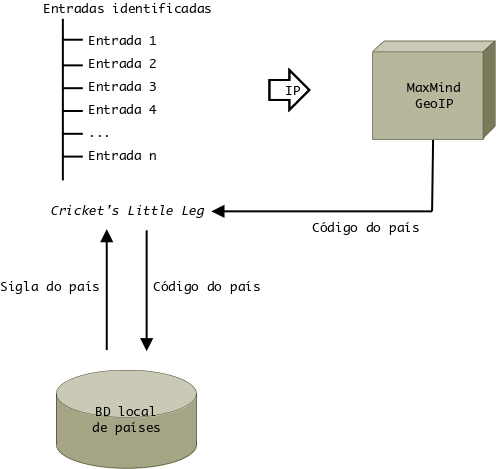
\includegraphics[scale=0.5]{./figuras/ws-geoip.png}

        \caption{\label{figura:ws-geoip}Identificação da procedência dos ataques.}
    \end{center}
\end{figure}
